\documentclass[a11paper, 11pt]{article}

\usepackage{document}
\usepackage{titlepage}
% Allows to include standalone files as figures
\usepackage{graphicx}
\usepackage{float}
\usepackage{pgf-umlcd}
\usepackage[T1]{fontenc}
\usepackage[french]{babel}
\usepackage{csquotes}
\usepackage{booktabs}
\usepackage{longtable}
\usepackage{xcolor}

% \addbibresource{bibliography.bib}
\nofiles

% Petites commandes utiles pour prendres des notes assez visibles
% pour être enlevées facilement
\newcommand{\note}[1]{\textbf{\textcolor{orange}{Note: #1}}}
\newcommand{\todo}[1]{\textbf{\textcolor{teal}{TODO: #1}}}
\newcommand{\fixme}[1]{\textbf{\textcolor{red}{FIXME: #1}}}

% \institution{Université de Sherbrooke}
% \faculty{Faculté de génie}
% \department{Département de génie électrique et de génie informatique}
\title{Rapport d'APP}
\classnb{GIF350}
\class{APP1 -- Modèles de conception}
\author{
  \addtolength{\tabcolsep}{-0.4em}
  \begin{tabular}{rcl} % Ajouter des auteurs au besoin
  Samuel Bilodeau  & -- & BILS2704 \\ % TODO: demander le CIP
  Benjamin Chausse & -- & CHAB1704 \\
  \end{tabular}
}
\teacher{Domingo Palao Munoz}
% \location{Sherbrooke}
% \date{\today}

\begin{document}
\maketitle
\newpage
\tableofcontents
\newpage
\section{Diagrammes de classes de \textit{MenuFact02}}

\fixme{Enlever le commentaire nofile avant de remettre le projet.}

\begin{figure}[H]
  \centering
  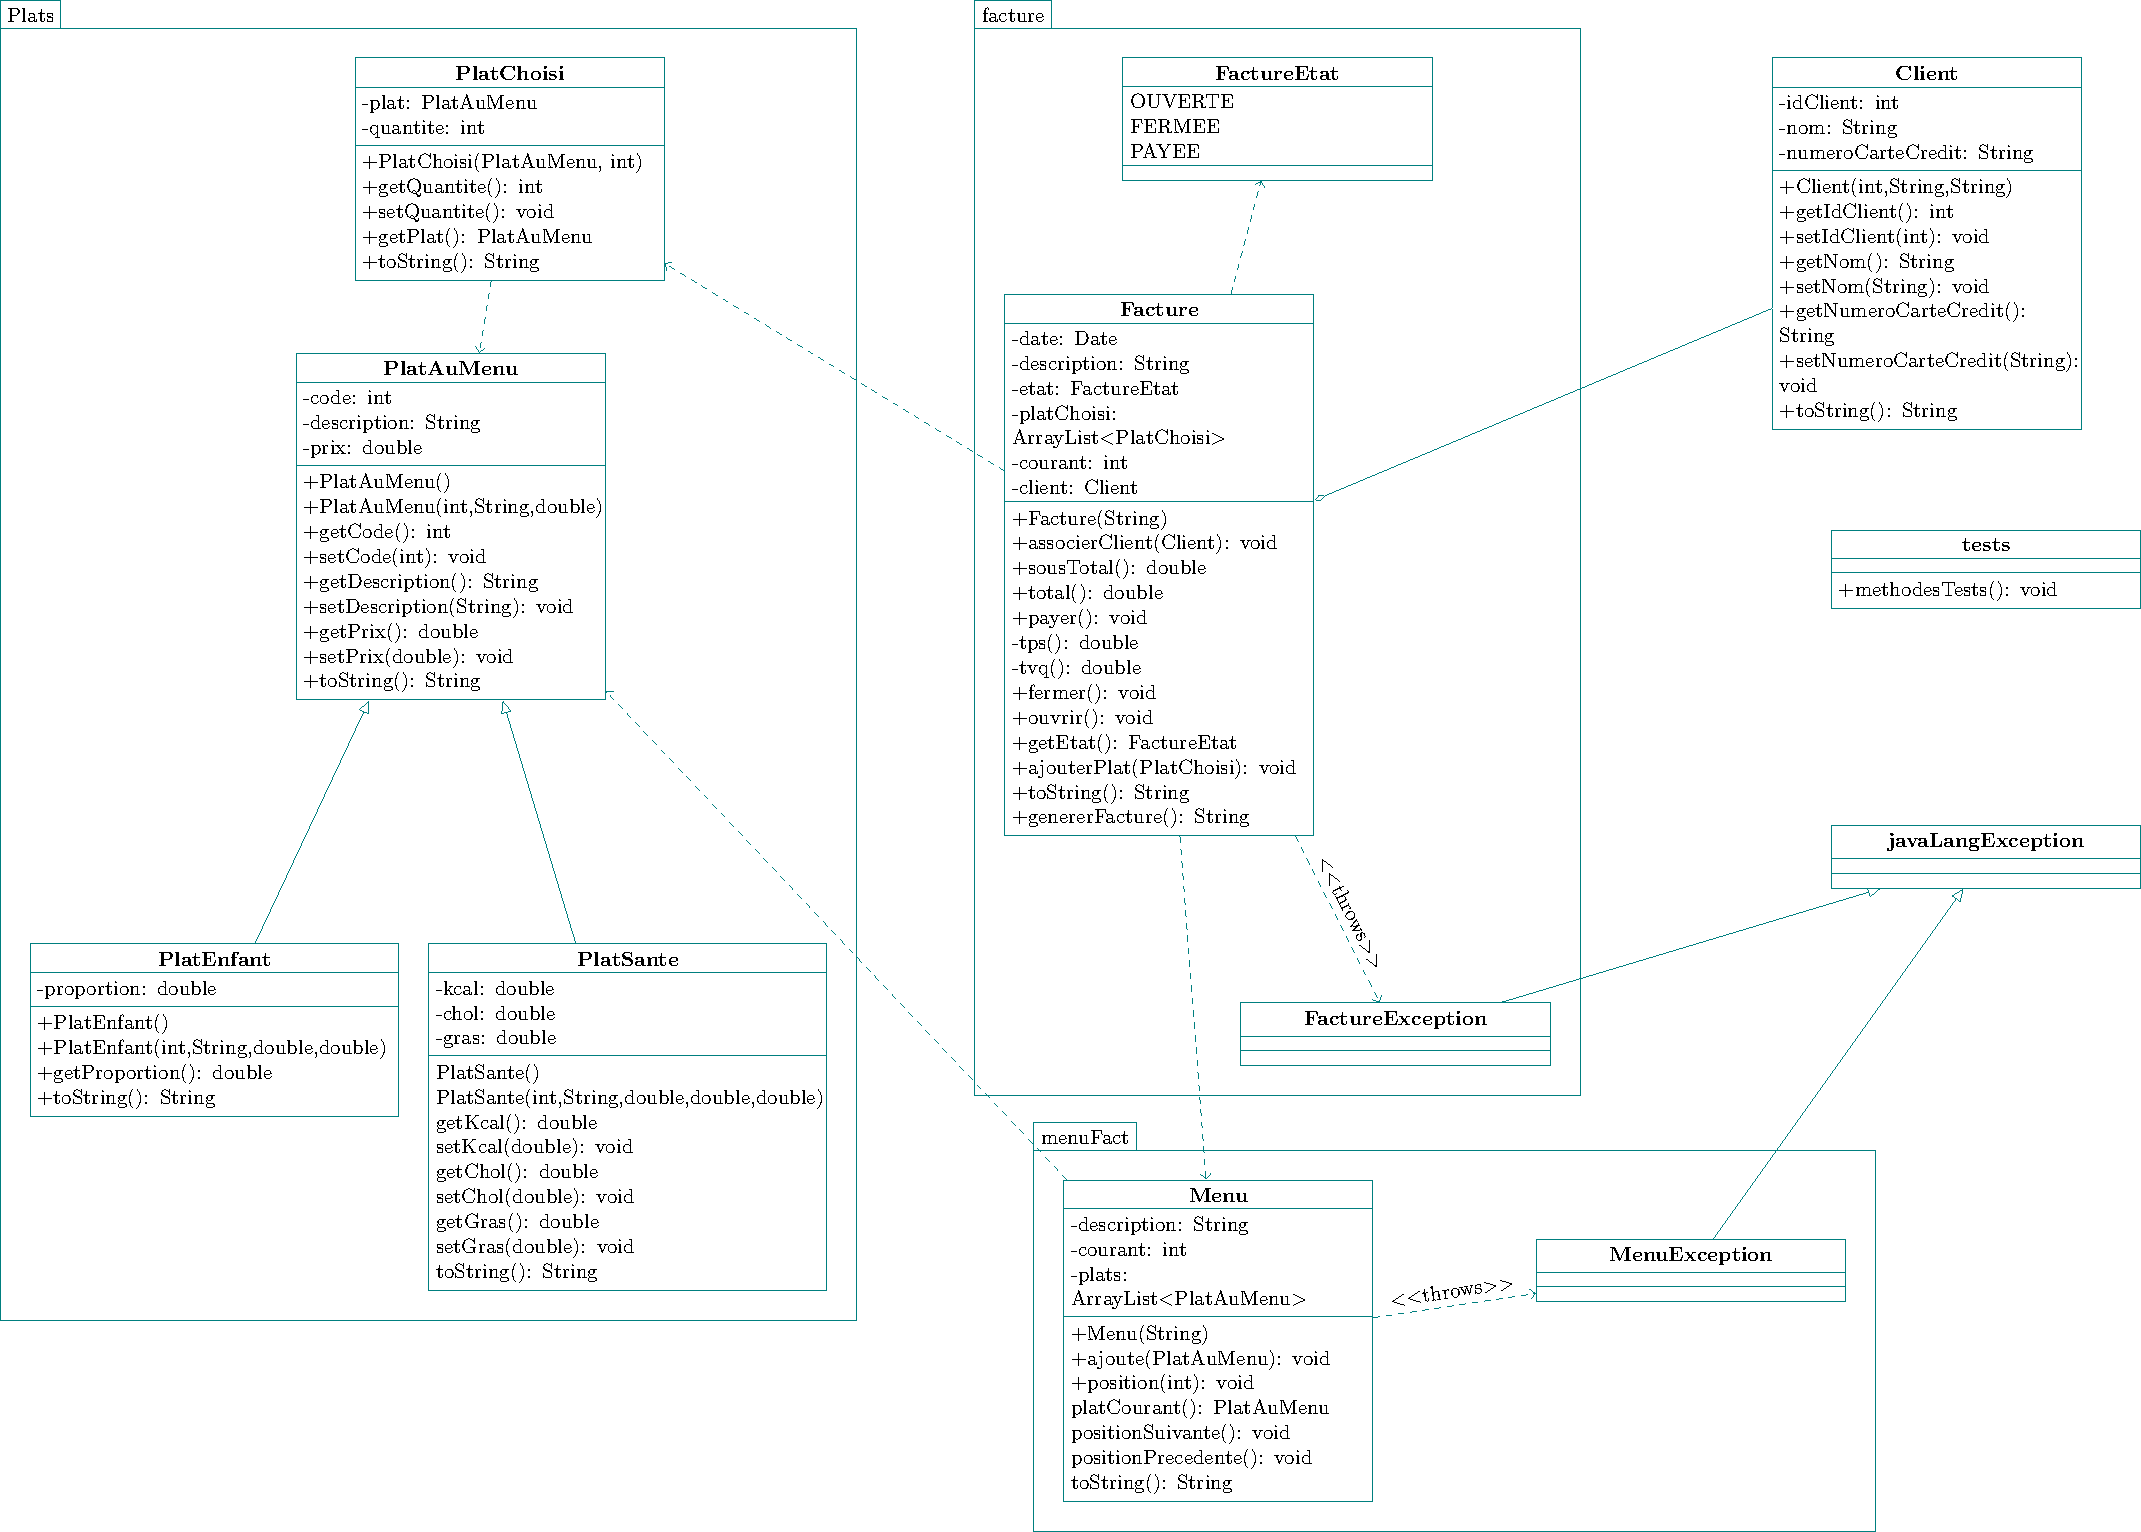
\includegraphics[width=\textwidth]{uml/uml.pdf}
  \caption{Diagramme de classes}
  \label{fig:uml}
\end{figure}

\section{Choix de conception}

\begin{table}[H]
\caption{Justification des modèles de conception}
\begin{longtable}{lp{10cm}}
\toprule
\textbf{Modèle de conception} & \textbf{Justification} \\

\midrule
Modèle-vue-contrôleur (MVC) &
Permet de séparer la logique de l'application, l'interface, et l'information
stockée par l'application. \verb|Terminal| est la vue (peut être changée pour
une interface web ou graphique sans changer la logique) , \verb|Controller| est
le cerveau de l'application et \verb|DataBroker| est le modèle qui stoque le Menu,
les factures, les Clients, les Chefs, etc\ldots \\

\midrule
Flyweight &
Permet de réduire la mémoire utilisée par l'application en
partageant le prix de tout les plat d'une même gamme de prix. (voir section
\ref{flyweight-notes}) \\

\midrule
States &
Permet de gérer l'état des factures. Une facture peut être
dans l'état Ouverte, Fermée ou Annulée. L'état détermine les actions possibles.
Par exemple, il est impossible d'ajouter des plats à une facture fermée. \\

\midrule
Observer &
La classe \verb|IngredientWatcher| permet de notifier les classes qui s'y
abonnent à chaque fois que les quantitées de divers ingrédients passent sous un
seuil critique. Par exemple, le \verb|Controller| pourrait s'abonner à cette
classe pour retirer du menu les plats qui ne peuvent plus être préparés. \\

\midrule
Factory&
La classe \verb|PlatFactory| permet de créer le bon type de plat selon les
paramètres qui lui sont passés. Par exemple, si les ingrédients utilisés sont
santé, la factory va créer un \verb|PlatSante|. Dans le cas où les proportions
sont petites, la factory va créer un \verb|PlatEnfant|. La gamme de prix est
aussi déterminée par les ingrédients utilisés. \\

\midrule
Singleton&

Diverses classes sont implémentées en tant que \verb|Singleton| pour éviter
divers problèmes de conception. Par exemple, il n'y a qu'un seul \verb|Menu|
pour tout le restaurant (deux clients ne devrait pas avoir deux menus
différents). Il n'y a qu'un seul \verb|DataBroker| pour gérer les données
globales de l'application. On ne veut pas avoir deux bases de données
différentes pour l'application. Finallement, il n'y a qu'un seul
\verb|Controller| pour gérer l'application. On veut éviter des problèmes de
synchronisation où deux contrôlleurs modifient la même information
simultanément. Cela n'empêche pas l'application d'avoir plusieurs
\verb|Terminal|s qui sont en communication avec le même \verb|Controller|. \\

\bottomrule

\end{longtable}
\end{table}


\subsection{Note sur l'utilisation du \textit{Flyweight}}
\label{flyweight-notes}

\note{Je sais pas si créer une section juste pour ça est une bonne idée.}

Comme mentionné lors du turorat, l'utilisation de patrons de conception était
surchargée pour le projet. On nous a demandé de les implémenter pricipalement à
des fins éducationnelles. Ceci dit, pour implémenter le patron
\textit{Flyweight}, nous avons pensé à l'idée d'un restaurant dans lequel les
Plats sont regroupés par gammes de prix (écono, régulier, deluxe). Ainsi,
chaque gamme de prix détient un \textit{flyweights} contenant le prix unique de
tout les plats dans cette gamme. Une économie de mémoire est donc réalisée
puisque la valeur du prix n'est pas dupliquée pour chaque plat d'une même
gamme. Bien sûr, une implémentation réaliste de ce patron contiendrait
généralement plus qu'un seul attribut dans le \textit{flyweights}. Ces classes
seraient donc nommées comme suit:

\begin{itemize}
  \item \verb|Flyweight|: Classe abstraite
  \item \verb|EconoFlyweight|: Classe concrète
  \item \verb|RegularFlyweight|: Classe concrète
  \item \verb|DeluxeFlyweight|: Classe concrète
\end{itemize}

\section{Utilité des modèles de conception}

\todo{Écrire cette section}

\section{Utilité des tests unitaires}

\todo{Écrire cette section}

% \newpage
% \printbibliography[heading=bibintoc]
\end{document}
